\chapter{Auswahl des Materials}

\begin{figure}[h]
  \centering
  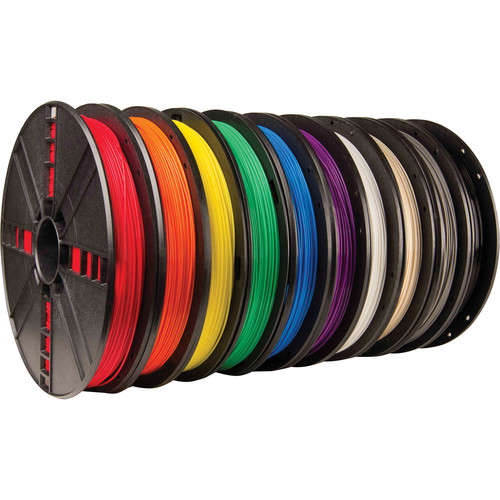
\includegraphics[width=10cm]{kapitel2/filament}
  \caption{Filamentspulen}
  \source{\url{https://www.bhphotovideo.com/c/product/1070383-REG/makerbot_mp06572_1_75mm_pla_filament_large.html}}
  \label{Kap2:Filament}
\end{figure}

\section{PLA}
\ac{PLA} ist das gängigste Material im 3D-Druck Hobbybereich bei einer Drucktemperatur von ca. 205\degree C. Aufgrund seiner Eigenschaften\footnote{PLA Materialeigenschaften nach \cite{ulPLA}} ist es sehr einfach schon in jedem Einsteiger-3D-Drucker zu verarbeiten. Es ist vergleichsweise leicht und umweltfreundlich, da es nicht aus Erdöl hergestellt wird und biologisch schneller abbaubar ist als andere Kunststoffe\footnote{Nach \cite{10093722}}. Auch ist es durch die weite Verbreitung gerade im 3D-Druck Bereich sehr günstig.
Punkte die gegen den Einsatz von \ac{PLA} sprechen sind hingegen die schwache mechanische Belastbarkeit und Temperaturstabilität, da \ac{PLA} nach der \ac{VST} nur bis ca. 54\degree C fest ist. Außerhalb des 3D-Druckes wird \ac{PLA} vor allem für Verpackungen eingesetzt, da hier die mechanische Belastbarkeit eine untergeordnete Rolle spielt und die Umweltfreundlichkeit im Vordergrund steht.

\begin{figure}[h]
  \centering
  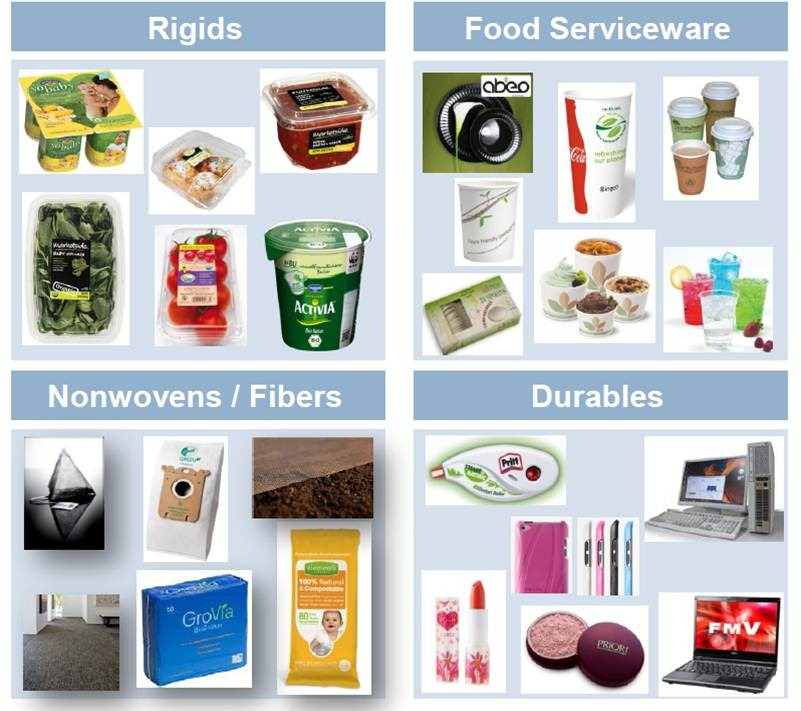
\includegraphics[width=10cm]{kapitel2/pla}
  \caption{Nutzungsgebiete von PLA}
  \source{\url{https://polymerinnovationblog.com/poly-lactic-acid-pla-is-gaining-traction-in-the-market/}}
  \label{Kap2:PLAEinsatz}
\end{figure}

\section{ABS}
Neben \ac{PLA} ist \ac{ABS} ein weiteres gängiges Material, welches jedoch vor allem im Profi-Bereich eingesetzt wird, da dort die Materialanforderungen häufig höher sind und es aufgrund seiner Eigenschaften\footnote{ABS Materialeigenschaften nach \cite{ulABS}} höhere Anforderungen an den 3D-Drucker stellt.

\TODO

\begin{figure}[h]
  \centering
  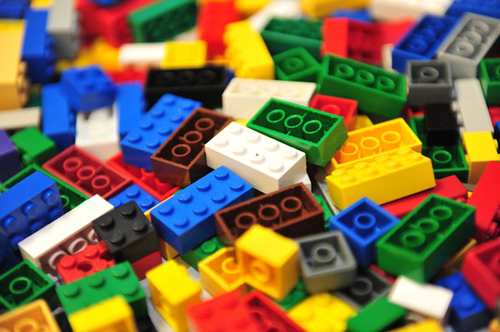
\includegraphics[width=10cm]{kapitel2/abs}
  \caption{LEGO-Bausteine aus ABS}
  \source{\url{https://27gen.com/2016/04/06/lego-bricks-toys-for-kids-lessons-for-adults/}}
  \label{Kap2:ABSLego}
\end{figure}